\documentclass[a4paper, 11pt]{article}
\usepackage{amsmath, amssymb, amsthm, amsfonts, tikz}
\usepackage[margin=1in]{geometry}
\usepackage{graphicx, pgfplots, booktabs, float}
\usetikzlibrary{intersections}

\pgfplotsset{compat=1.17}

\title{Machine Learning Homework \\SVM \& Kernels}
\author{Vahid Maleki}
\date{\today}

\begin{document}
	\maketitle
	\section{Question One}
	
	Given the mapping 
	\[
	x \in \mathbb{R} \to y \equiv \varphi(x) \in \mathbb{R}^{2k+1}
	\]
	where
	\[
	\varphi(x) = 
	\begin{bmatrix} 
		\frac{1}{\sqrt{2}} & \cos x & \cos 2x & \cdots & \cos kx & \sin x & \sin 2x & \cdots & \sin kx 
	\end{bmatrix}^T
	\]
	we need to show that the inner product kernel is given by:
	\[
	k(x_i, x_j) = y_i^T y_j = \frac{\sin((k + 0.5)(x_i - x_j))}{2\sin\left(\frac{x_i - x_j}{2}\right)}.
	\]
	\subsection*{Solution}
	The inner product $y_i^T y_j$ is the dot product of the vectors $\varphi(x_i)$ and $\varphi(x_j)$:
	\[
	y_i^T y_j = \varphi(x_i)^T \varphi(x_j).
	\]
	Substituting the expression for $\varphi(x)$, we have:
	\[
	\varphi(x_i)^T \varphi(x_j) = \left(\frac{1}{\sqrt{2}}\right)^2 + \sum_{n=1}^k \cos(nx_i)\cos(nx_j) + \sum_{n=1}^k \sin(nx_i)\sin(nx_j).
	\]
	Simplifying, the first term is:
	\[
	\left(\frac{1}{\sqrt{2}}\right)^2 = \frac{1}{2}.
	\]
	Using the trigonometric identity $\cos A \cos B + \sin A \sin B = \cos(A - B)$, the remaining terms become:
	\[
	\sum_{n=1}^k \cos(nx_i)\cos(nx_j) + \sum_{n=1}^k \sin(nx_i)\sin(nx_j) = \sum_{n=1}^k \cos(n(x_i - x_j)).
	\]
	Thus, we have:
	\[
	y_i^T y_j = \frac{1}{2} + \sum_{n=1}^k \cos(n(x_i - x_j)).
	\]
	The summation $\sum_{n=1}^k \cos(n(x_i - x_j))$ is a geometric series. Let $\Delta = x_i - x_j$. Then:
	\[
	\sum_{n=1}^k \cos(n\Delta) = \text{Re} \left( \sum_{n=1}^k e^{in\Delta} \right).
	\]
	The sum of a geometric series is given by:
	\[
	\sum_{n=1}^k e^{in\Delta} = \frac{e^{i\Delta}(1 - e^{ik\Delta})}{1 - e^{i\Delta}}.
	\]
	Taking the real part, we have:
	\[
	\sum_{n=1}^k \cos(n\Delta) = \text{Re} \left( \frac{e^{i\Delta}(1 - e^{ik\Delta})}{1 - e^{i\Delta}} \right).
	\]
	Using $e^{i\theta} = \cos\theta + i\sin\theta$, we simplify:
	\[
	\sum_{n=1}^k \cos(n\Delta) = \frac{\sin(k\Delta/2)\cos((k+0.5)\Delta)}{\sin(\Delta/2)}.
	\]
	Thus, the inner product becomes:
	\[
	y_i^T y_j = \frac{1}{2} + \frac{\sin(\frac{k\Delta}{2})\cos((k+0.5)\Delta)}{\sin(\frac{\Delta}{2})}.
	\]
	Using the trigonometric identity $\sin(A) + \sin(B) = 2\sin\left(\frac{A+B}{2}\right)\cos\left(\frac{A-B}{2}\right)$, the kernel simplifies to:
	\[
	y_i^T y_j = \frac{1}{2} + \frac{\frac{1}{2} \left[ \sin\left((k+0.5)\Delta\right) - \sin\left(\frac{\Delta}{2}\right) \right]}{\sin(\frac{\Delta}{2})}.
	\]
	know we can distrbute the fraction:
	\[ 
	y_i^T y_j = \frac{1}{2} + \frac{\sin((k+0.5)\Delta)}{2\sin(\frac{\Delta}{2})} - \frac{\sin(\frac{\Delta}{2})}{2\sin(\frac{\Delta}{2})} 
	\]
	after substituding $\Delta$ with $x_i - x_j$ we complete the proof:
	\[
	k(x_i, x_j) = y_i^T y_j = \frac{\sin((k + 0.5)(x_i - x_j))}{2\sin\left(\frac{x_i - x_j}{2}\right)}.
	\]
	
	\newpage
	\section{Question Two}
	
	
	Two one-dimensional classification tasks are given. We will analyze each case separately.
	
	\subsection*{Part (a)}
	The data points for part (a) are as follows:
	
	\[
	\begin{array}{|c|c|}
		\hline
		x & y = d \\
		\hline
		2 & 1 \\
		-1 & -1 \\
		-2 & -1 \\
		1 & 1 \\
		\hline
	\end{array}
	\]\\\\
	Below is the plot of the data points in the $(x, y)$ plane:
	
	\begin{center}
		\begin{tikzpicture}
			\begin{axis}[
				axis lines = middle,
				xlabel = {$x$},
				ylabel = {$y$},
				ymin = -1.5, ymax = 1.5,
				xmin = -3, xmax = 3,
				xtick = {-2, -1, 0, 1, 2},
				ytick = {-1, 1},
				grid = both,
				grid style = {dashed, gray!30}
				]
				\addplot[only marks, mark=*, red] coordinates {(2,1) (1,1)};
				\addplot[only marks, mark=square*, blue] coordinates {(-1,-1) (-2,-1)};
			\end{axis}
		\end{tikzpicture}
	\end{center}
	The optimal canonical hyperplane maximizes the margin between the two classes. The support vectors for this dataset are $x = 1$ and $x = -1$.\\\\
	The decision boundary is the midpoint of the margin between the support vectors:
	\[
	x = 0.
	\]
	The canonical hyperplane equation is:
	\[
	w \cdot x + b = 0,
	\]
	where $w = 1$ and $b = 0$. Therefore:
	\[
	x = 0.
	\]
	
	\begin{center}
		\begin{tikzpicture}
			\begin{axis}[
				axis lines = middle,
				xlabel = {$x$},
				ylabel = {$y$},
				ymin = -1.5, ymax = 1.5,
				xmin = -3, xmax = 3,
				xtick = {-2, -1, 0, 1, 2},
				ytick = {-1, 1},
				grid = both,
				grid style = {dashed, gray!30}
				]
				% Data points for Class +1
				\addplot[only marks, mark=*, red] coordinates {(2,1) (1,1)};
				% Data points for Class -1
				\addplot[only marks, mark=square*, blue] coordinates {(-1,-1) (-2,-1)};
				% Decision boundary x = 0
				\addplot[domain=-1.5:1.5, samples=2, color=violet, thick, dashed] coordinates {(0,-1.5) (0,1.5)} 
				node[midway, right] {x = 0};
			\end{axis}
		\end{tikzpicture}
	\end{center}
	
	\subsection*{Part (b)}
	The data points for part (b) are as follows:
	
	\[
	\begin{array}{|c|c|}
		\hline
		x & y = d \\
		\hline
		3 & 1 \\
		1 & -1 \\
		-1 & -1 \\
		\hline
	\end{array}
	\]
	Below is the plot of the data points in the $(x, y)$ plane:
	
	\begin{center}
		\begin{tikzpicture}
			\begin{axis}[
				axis lines = middle,
				xlabel = {$x$},
				ylabel = {$y$},
				ymin = -1.5, ymax = 1.5,
				xmin = -2, xmax = 4,
				xtick = {-1, 0, 1, 2, 3},
				ytick = {-1, 1},
				grid = both,
				grid style = {dashed, gray!30}
				]
				\addplot[only marks, mark=*, red] coordinates {(3,1)};
				\addplot[only marks, mark=square*, blue] coordinates {(1,-1) (-1,-1)};
			\end{axis}
		\end{tikzpicture}
	\end{center}
	The support vectors for this dataset are $x = 3$ (class $1$) and $x = 1$ (class $-1$).
	\\\\
	The decision boundary is the midpoint of the margin between the support vectors:
	\[
	x = 2.
	\]
	The canonical hyperplane equation is:
	\[
	w \cdot x + b = 0,
	\]
	where $w = 1$ and $b = -2$. Therefore:
	\[
	x - 2 = 0 \quad \text{or} \quad x = 2.
	\]
	\begin{center}
		\begin{tikzpicture}
			\begin{axis}[
				axis lines = middle,
				xlabel = {$x$},
				ylabel = {$y$},
				ymin = -1.5, ymax = 1.5,
				xmin = -2, xmax = 4,
				xtick = {-1, 0, 1, 2, 3},
				ytick = {-1, 1},
				grid = both,
				grid style = {dashed, gray!30}
				]
				\addplot[only marks, mark=*, red] coordinates {(3,1)};
				\addplot[only marks, mark=square*, blue] coordinates {(1,-1) (-1,-1)};
				\addplot[domain=-1.5:1.5, samples=2, color=violet, thick, dashed] coordinates {(2,-1.5) (2,1.5)} 
				node[midway, right] {x = 2};
			\end{axis}
		\end{tikzpicture}
	\end{center}
	
	\newpage
	\section{Question Three}
	Classify two one-dimensional data points using Support Vector Machine (SVM) with a first-order polynomial kernel. The data points and their labels are:
	\begin{itemize}
		\item $x_1 = -1$, $y_1 = -1$
		\item $x_2 = 1$, $y_2 = +1$
	\end{itemize}
	
	\subsection*{Solution}
	We are using a first-order polynomial kernel, which is given by:
	\[
	K(x_i, x_j) = (x_i \cdot x_j + c)^d
	\]
	For a first-order polynomial kernel ($d=1$) and assuming $c=0$, the kernel simplifies to:
	\[
	K(x_i, x_j) = x_i \cdot x_j
	\]
	

	\noindent The kernel matrix $K$ is computed as follows:
	\[
	K = 
	\begin{bmatrix}
		K(x_1, x_1) & K(x_1, x_2) \\
		K(x_2, x_1) & K(x_2, x_2)
	\end{bmatrix}
	\]
	Substitute the values of $x_1 = -1$ and $x_2 = 1$:
	\[
	K(x_1, x_1) = (-1) \cdot (-1) = 1
	\]
	\[
	K(x_1, x_2) = (-1) \cdot 1 = -1
	\]
	\[
	K(x_2, x_1) = 1 \cdot (-1) = -1
	\]
	\[
	K(x_2, x_2) = 1 \cdot 1 = 1
	\]
	Thus, the kernel matrix is:
	\[
	K = 
	\begin{bmatrix}
		1 & -1 \\
		-1 & 1
	\end{bmatrix}
	\]\\\\
	The dual form of the SVM optimization problem is:
	\[
	\max_{\alpha} \left( \sum_{i=1}^{n} \alpha_i - \frac{1}{2} \sum_{i=1}^{n} \sum_{j=1}^{n} \alpha_i \alpha_j y_i y_j K(x_i, x_j) \right)
	\]
	Subject to:
	\[
	\sum_{i=1}^{n} \alpha_i y_i = 0 \quad \text{and} \quad \alpha_i \geq 0
	\]
	Substitute $n=2$, $y_1 = -1$, $y_2 = +1$, and the kernel matrix values:
	\[
	\max_{\alpha_1, \alpha_2} \left( \alpha_1 + \alpha_2 - \frac{1}{2} \left[ \alpha_1^2 + \alpha_2^2 - 2\alpha_1 \alpha_2 \right] \right)
	\]
	Subject to:
	\[
	-\alpha_1 + \alpha_2 = 0 \quad \text{and} \quad \alpha_1, \alpha_2 \geq 0
	\]
	\\
	From the constraint $-\alpha_1 + \alpha_2 = 0$, we get $\alpha_2 = \alpha_1$. Substitute this into the objective function:
	\[
	\max_{\alpha_1} \left( 2\alpha_1 - \frac{1}{2} \left[ 2\alpha_1^2 \right] \right)
	\]
	Simplify:
	\[
	\max_{\alpha_1} \left( 2\alpha_1 - \alpha_1^2 \right)
	\]
	Take the derivative and set it to zero:
	\[
	\frac{d}{d\alpha_1} \left( 2\alpha_1 - \alpha_1^2 \right) = 2 - 2\alpha_1 = 0
	\]
	Thus, $\alpha_1 = 1$, and therefore $\alpha_2 = 1$.
	\\

	\noindent The decision function is:
	\[
	f(x) = \sum_{i=1}^{n} \alpha_i y_i K(x_i, x) + b
	\]
	Substitute the known values:
	\[
	f(x) = \alpha_1 y_1 K(x_1, x) + \alpha_2 y_2 K(x_2, x) + b
	\]
	\[
	f(x) = (1)(-1)(-x) + (1)(+1)(x) + b
	\]
	\[
	f(x) = 2x + b
	\]
	To find $b$, use the condition that for a support vector $f(x_i) = y_i$:
	\[
	f(-1) = -1 \quad \Rightarrow \quad 2(-1) + b = -1 \quad \Rightarrow \quad b = 1
	\]
	Thus, the decision boundary is:
	\[
	f(x) = 2x + 1
	\]
	
	\newpage
	\section*{Question Four}
	Minimize the function:
	\[
	f(x_1, x_2) = (x_1 - 1)^2 + (x_2 - 2)^2
	\]
	subject to the following constraints:
	\begin{align*}
		g_1(x_1, x_2) &= x_2 - x_1 - 1 = 0 \\
		g_2(x_1, x_2) &= x_2 + x_1 - 2 \le 0 \\
		g_3(x_1) &= -x_1 \le 0 \\
		g_4(x_2) &= -x_2 \le 0
	\end{align*}
	
	\subsection*{Solution}
	The Lagrangian for this problem is:
	\[
	\mathcal{L}(x_1, x_2, \lambda_1, \lambda_2, \mu_1, \mu_2) = (x_1 - 1)^2 + (x_2 - 2)^2 + \lambda_1 (x_2 - x_1 - 1) + \lambda_2 (x_2 + x_1 - 2) + \mu_1 (-x_1) + \mu_2 (-x_2)
	\]
	where $\lambda_1, \lambda_2 \ge 0$ and $\mu_1, \mu_2 \ge 0$.
	
	\subsection*{Stationarity Conditions}
	\[
	\frac{\partial \mathcal{L}}{\partial x_1} = 2(x_1 - 1) - \lambda_1 + \lambda_2 - \mu_1 = 0
	\]
	\[
	\frac{\partial \mathcal{L}}{\partial x_2} = 2(x_2 - 2) + \lambda_1 + \lambda_2 - \mu_2 = 0
	\]
	
	\subsection*{Complementary Slackness}
	\begin{align*}
		\lambda_1 (x_2 - x_1 - 1) &= 0 \\
		\lambda_2 (x_2 + x_1 - 2) &= 0 \\
		\mu_1 x_1 &= 0 \\
		\mu_2 x_2 &= 0
	\end{align*}
	
	\subsection*{Solve the System of Equations}
	Consider each constraint and solve the corresponding system of equations.
	
	\paragraph{Case 1: $x_1, x_2 > 0$}
	This implies $\mu_1 = 0$ and $\mu_2 = 0$. Assume $\lambda_2 = 0$ (since $x_2 + x_1 - 2 \neq 0$).
	
	Simplify the stationarity conditions:
	\[
	2(x_1 - 1) - \lambda_1 = 0 \quad \Rightarrow \quad \lambda_1 = 2(x_1 - 1)
	\]
	\[
	2(x_2 - 2) + \lambda_1 = 0 \quad \Rightarrow \quad 2(x_2 - 2) + 2(x_1 - 1) = 0
	\]
	This gives:
	\[
	x_2 + x_1 = 4
	\]
	Combine with $x_2 - x_1 = 1$, solving:
	\[
	x_1 = \frac{3}{2}, \quad x_2 = \frac{5}{2}
	\]
	
	\paragraph{Case 2: Check Boundary Constraints}
	Verify which of the constraints are active at the solution $(\frac{3}{2}, \frac{5}{2})$. Since this violates $x_2 + x_1 \le 2$, we check the boundaries.
	
	\subsection*{Graphical Verification}
	The feasible region is defined by the following constraints:
	\begin{itemize}
		\item $x_2 - x_1 = 1$
		\item $x_2 + x_1 \le 2$
		\item $x_1, x_2 \ge 0$
	\end{itemize}
	
	\begin{figure}[h]
		\centering
		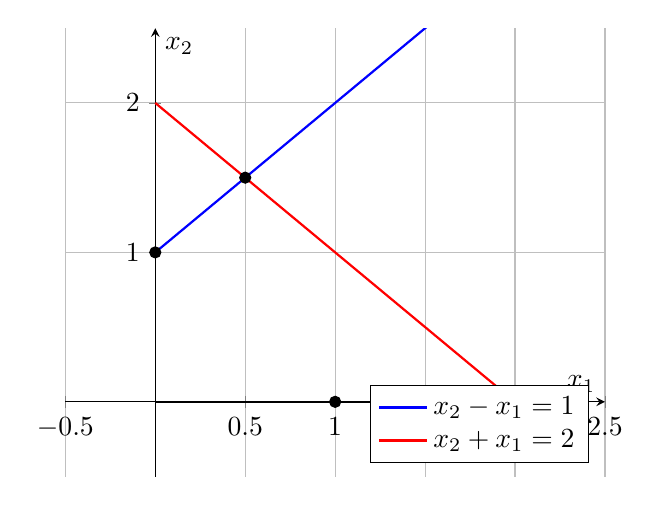
\begin{tikzpicture}
			\begin{axis}[
				axis lines=middle,
				xlabel={$x_1$},
				ylabel={$x_2$},
				xmin=-0.5, xmax=2.5,
				ymin=-0.5, ymax=2.5,
				grid=both,
				legend pos=south east
				]
				% Feasible region
				\addplot[name path=constraint1, domain=0:2, samples=100, thick, blue] {x+1};
				\addplot[name path=constraint2, domain=0:2, samples=100, thick, red] {2-x};
				\addplot[name path=xaxis, domain=0:2, samples=2, thick] {0};
				
				% Intersection points
				\addplot[mark=*, only marks] coordinates {(0.5,1.5) (0,1) (1,0)};
				
				\legend{$x_2 - x_1 = 1$, $x_2 + x_1 = 2$}
			\end{axis}
		\end{tikzpicture}
		\caption{Feasible region and constraints.}
	\end{figure}
	
	\newpage
	\section*{Question Five}
	This report presents the results of using Support Vector Machines (SVM) with different kernels—linear, polynomial, and radial basis function (RBF)—to classify the Sonar dataset. The dataset was randomly split into 80\% for training and 20\% for testing. The performance of each model was evaluated in terms of accuracy on both the training and test sets.
	
	\subsection*{Data Preparation}
	\begin{itemize}
		\item The Sonar dataset was loaded and split into features (\(X\)) and target labels (\(y\)).
		\item Target labels were encoded using \texttt{LabelEncoder}, converting categorical labels ('R' and 'M') into numerical format.
		\item The dataset was split into training (80\%) and test (20\%) sets using \texttt{train\_test\_split} with stratification to maintain label distribution.
		\item The features were standardized using \texttt{StandardScaler} to ensure all input dimensions had zero mean and unit variance.
	\end{itemize}
	
	\subsection*{Model Training and Evaluation}
	The following SVM models were trained and evaluated:
	\begin{itemize}
		\item \textbf{Linear Kernel:} A basic linear SVM was trained with default parameters.
		\item \textbf{Polynomial Kernel:} A polynomial SVM with degree 3 was used.
		\item \textbf{RBF Kernel:} An SVM with an RBF kernel and \(C = 1\) was trained.
	\end{itemize}
	
	The models were evaluated using the accuracy score on both the training and test sets. The key parts of the Python code used are:
	
	\begin{verbatim}
		# Linear SVM
		model = SVC(kernel='linear', C=1)
		model.fit(X_train, y_train)
		train_acc = accuracy_score(y_train, model.predict(X_train))
		test_acc = accuracy_score(y_test, model.predict(X_test))
		
		# Polynomial Kernel SVM (degree 3)
		model = SVC(kernel='poly', degree=3, C=1)
		
		# RBF Kernel SVM
		model = SVC(kernel='rbf', C=1)
	\end{verbatim}
	\newpage
	\section*{Results}
	The following table summarizes the classification accuracy of the SVM models on the training and test sets:
	
	\begin{table}[H]
		\centering
		\begin{tabular}{@{}lccc@{}}
			\toprule
			\textbf{SVM Kernel} & \textbf{Kernel Parameter Value} & \textbf{Train Accuracy} & \textbf{Test Accuracy} \\
			\midrule
			Linear             & -                               & 0.9518                  & 0.7619                  \\
			Polynomial (degree 3) & 3                            & 0.9879                  & 0.7857                  \\
			RBF                & \(C=1\)                         & 0.9940                  & 0.8571                  \\
			\bottomrule
		\end{tabular}
		\caption{SVM Classification Results}
	\end{table}
	

	The RBF kernel achieved the highest test accuracy (85.71\%), followed by the polynomial kernel (78.57\%) and the linear kernel (76.19\%). This suggests that the RBF kernel can capture complex decision boundaries better than the linear and polynomial kernels. However, the slight overfitting observed in the RBF model (with near-perfect training accuracy) indicates a potential need for further hyperparameter tuning.
	\\\\
	The differences in results compared to those reported in external sources may arise from:
	\begin{itemize}
		\item The random splitting of the dataset into training and test sets.
		\item Differences in hyperparameter settings such as the value of \(C\) or kernel parameters.
		\item Variations in feature preprocessing or scaling techniques.
	\end{itemize}
\end{document}
